\documentclass[a4paper,titleauthor]{mwart} 

\usepackage{polski}
\usepackage[utf8]{inputenc}
\usepackage{graphicx} %pakiet do wstawiania grafiki
\usepackage[hyphens]{url} %pakiet do wstawiania linkow
%\usepackage[hidelinks,breaklinks]{hyperref}
\usepackage{authblk}%pakiet do tworzenia afiliacji
\usepackage{tabularx}%pakiet do tabel
\usepackage[a4paper, left=2cm, right=2cm, top=3cm, bottom=3cm]{geometry}
\usepackage{listings}
\usepackage{placeins}%pakiet do kontroli umieszczania obiektow
\usepackage{hyperref}%pakiet do m.in. kolorowania linkow

\usepackage[tablegrid,owncaptions]{vhistory}
\renewcommand{\vhhistoryname}{Historia zmian}
\renewcommand{\vhversionname}{Wersja}
\renewcommand{\vhdatename}   {Data}
\renewcommand{\vhauthorname} {Autor}
\renewcommand{\vhchangename} {Opis zmian}

\renewcommand\figurename{Rys.}%skrocony podpis
\renewcommand\lstlistingname{Wydruk}


%------------------------------------------------------------------------
% Dane do strony tytułowej

\title{{\Huge  Projekt SYCYF}\\ - \\{\Large Zespół nr 6}\\ }

\author{Sofiia Levchenko \and Joanna Stalenczyk \and Julia Boryslawska \and Jakub Tarczynski \and Jan Zobniow}

\date{\today}

%------------------------------------------------------------------------
% Początek dokumentu
\begin{document}

%Automatycznie generowany tytuł dokumentu
\maketitle
%------------------------------------------------------------------------
% Automatycznie generowany spis treści
\tableofcontents

%------------------------------------------------------------------------
\section{Wstęp}
\label{sec:wstep}%etykieta

Raport bedzie dokumentowany \textbf{przyrostowo} zgodnie z realizacja projektu. Poszczególne etapy realizacji projektu obejmują: 

\renewcommand{\labelenumi}{\Roman{enumi}}
\begin{enumerate}\setlength{\itemsep}{0.2\baselineskip} 
	\item Etap wstępny – stworzenie zespołu i organizacja warsztatu pracy, 
	\item Etap zdobywania informacji – analiza literatury, istniejących metod, zebranie wiedzy teoretycznej związanej z tematem projektu, 
	\item Etap opracowania koncepcji – szukanie rozwiązań, najlepiej sprawdzi się proces burzy mózgów (mapy myśli), opracowanie koncepcji rozwiązania  na podstawie zdobytej wiedzy, opracowanie prostego modelu referencyjnego (Python, MATLAB/GNU Octave, itp) i danych do testowania  
	\item Etap implementacji – na tym etapie rozwijamy i rozbudowujemy koncepcje projektowe docelowego systemu, modelujemy elementy systemu w HDL, weryfikujemy funkcjonalnie, integrujemy i oceniamy prototypy, 
	\item Etap uruchomienia – wdrożenie projektu, uruchomienie na docelowej platformie, przetestowanie według wcześniej opracowanych scenariuszy testowych. 
\end{enumerate}

Prace wykonane w ramach każdego etapu beda opisane w oddzielnych rozdziałach raportu.

\section{Organizacja prac}
\label{sec:organizacja}

Rozdział ten będzie opisywał zadania zrealizowane w ramach Etapu \texttt{I}. W tym rozdziale będą omówione:

\begin{itemize}
	\item analiza podejścia Design Thinking oraz trzech jego wersji (pięć kroków Design Thinkig'u, trzy zachodzące na siebie fazy procesu Design Thinking'u oraz cztero-fazowy proces "Double Dimond")
	\item wybor jedynego sposobu zarządzania projektem
	\item analiza różnego rodzaju narzędzi (TeXstudio, Overleaf, Microsoft Word, Microsoft Teams, Skype, GitHub oraz GitLab)
	\item organizacja warsztatu pracy, dobór narzędzi (Overleaf, Microsoft Teams, GutHub, itp.)
	\item ostateczny dobór narzędzi
	\item organizacja warsztatu pracy
\end{itemize}

\subsection{Design Thinking}
\label{sec:design_thinking}
Co to jest "Design Thinking?" \newline
\newline
Design thinking – jest to proces odnoszący się do procesów poznawczych, strategicznych i praktycznych, dzięki którym koncepcje projektowe (propozycje nowych produktów, usług itp.) są opracowywane przez projektantów i / lub zespoły projektowe~\cite{DesignThinking1}. \newline \newline Wiele osób próbowało sformalizować podstawowe zasady zastosowania myślenia projektowego w organizacjach, za pomocą modeli procesów i metodologii. Pomimo niekończących się modyfikacji i mutacji istnieją trzy, trwałe, ogólne przyjęte modele~\cite{DesignThinking2}:

 \begin{itemize}
 	\item Pięć kroków Design Thinkig'u
 	\item Trzy zachodzące na siebie fazy procesu Design Thinking'u
 	\item Cztero-fazowy proces "Double Dimond"
 \end{itemize}

Diagramy i słownictwo mogą się różnić, ale we wszystkich modelach myślenia projektowego występują wyraźne tematy:

 \begin{itemize}
	\item \textbf{Zorientowane na człowieka}\newline \newline Fazy odkrywania i inspiracji koncentrują się na badaniach proponowanego użytkownika - "Kim oni są?", "Czego chcą / potrzebują?", "Jak się zachowują?" Chodzi o budowanie empatii przez zespół projektowy z użytkownikiem końcowym i zrozumienie, dla kogo projektują.\newline
	\item \textbf{Iteracyjny} \newline \newline Fazy opracowywania, dostarczania i wdrażania skupiają się na usuwaniu najsłabszych pomysłów i ulepszaniu najsilniejszych poprzez prototypowanie, testowanie i optymalizację.\newline
	\item \textbf{Interdyscyplinarne} \newline \newline Wszystkie modele pokazują podróż, która rozbiega się i zbiega, przynajmniej w początkowe rozwiązanie. Każda faza nie jest własnością jednego zespołu z ustalonymi zadaniami; zamiast tego wspólny zespół projektowy wyrusza razem w podróż. Należy zauważyć, że zespoły interdyscyplinarne różnią się od zespołów multidyscyplinarnych tym, że każdy z nich ma wspólną odpowiedzialność za projekt i jego sukces, zamiast opowiadać się za własną specjalizacją.
 \end{itemize}

 \subsubsection{Zalety i wady Design Thinking'u}
Do głównych zalet należą:\newline
\begin{itemize}
\item Ułatwia i przyspiesza przyjęcie rozwiązania: dzięki takiemu podejściu projektowanie oparte na Design Thinking zaczyna się od potrzeby użytkownika końcowego, kończy na zbudowaniu rozwiązania (technologicznego lub procesowego), które jest dla niego naprawdę cenne.
\item Silne zaangażowanie użytkownika końcowego, który czuje się zaangażowany już od strony projektowej: sposób dla firm na ulepszenie swoich pracowników i „wzięcie ich na pokład” stojącego przed nimi wyzwania;
\item Iteracyjne podejście na etapie projektowania pozwala przetestować propozycje rozwiązań i modyfikować je, aż do osiągnięcia najbardziej odpowiedniego rozwiązania przed przystąpieniem do faktycznego wdrożenia;
\end{itemize}
\vspace{0,5cm}
\hspace{0,5cm}Wady Design Thinking'u:\newline
\begin{itemize}
\item Projekt moze trwać długo, a końcową werseję można zastosować tylko do ograniczonych celów
	\item Zastosowanie metodologii projektowania korporacyjnych rozwiązań cyfrowych może kolidować z ograniczeniami nałożonymi przez integrację z już używanymi rozwiazaniami.
	\item Myślenie projektowe wymaga bezpośredniego zaangażowania użytkowników, którzy muszą mieć możliwość wniesienia własnego wkładu (dostępność czasu i zasobów)
\end{itemize}
 

 \subsubsection{Pięć kroków Design Thinkig'u}
 Model ten składa się z 5 etapów: empatyzacji, definiowania problemu, kreatywnego myślenia, tworzenia prototypu, testowania.
\begin{figure}[h]
 	\centering
 	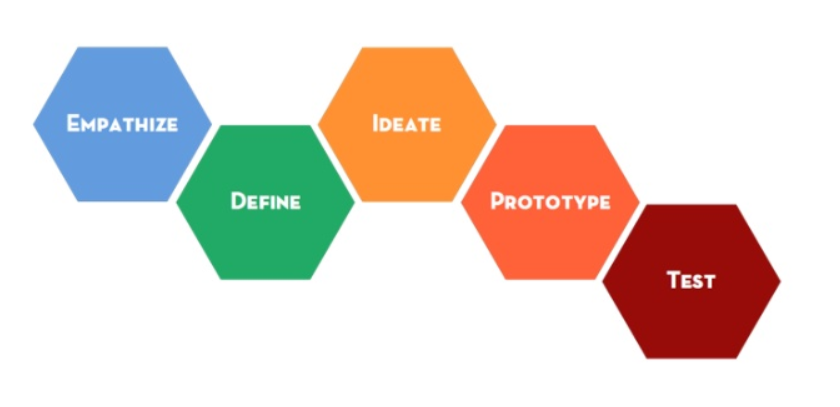
\includegraphics[width=0.8\textwidth]{5krokow.PNG}
 	\caption{Pięć kroków Design Thinkig'u}
 \end{figure}
 \begin{itemize}
     \item \textbf {Empatyzacja}\newline \newline
     W pierwszym kroku skupiamy się na człowieku, czyli odbiorcy naszego projektu. Staramy się zrozumieć czego potrzebuje, dlaczego tego potrzebuje, w jaki sposób będzie z tego korzystał. Robimy to, ponieważ często tworzymy innym, rozwiązujemy cudze problemy, przez co musimy je najpierw dobrze zrozumieć. \newline
     \item \textbf{Definiowanie problemu}\newline \newline
     Gdy już poznamy odbiorcę, naszym zadaniem jest odpowiednie zdefiniowanie problemu, odnalezienie czegoś przydatnego, czegoś co zaspokoi jego potrzeby. Jest to ważny etap, ponieważ od tego zależy nad czym dalej będziemy pracować.\newline \newline
     \item\textbf{Kreatywne myślenie}\newline \newline
     W następnym etapie podchodzimy do problemu jakby nie istniały żadne ograniczenia finansowe ani fizyczne, uruchamiamy kreatywne myślenie. W tym kroku nie zależy nam na odnalezieniu odpowiedniego rozwiązania, tylko na wymyśleniu jak najrozmaitszych pomysłów, co się przyczyni do innowacyjności projektu.\newline
     \item\textbf{Tworzenie prototypu}\newline \newline
     Następnie według tego modelu należy stworzyć prototyp. Powinien on być tani oraz szybki do zrobienia. Jego zadaniem jest ułatwienie wyobrażenia potencjalnych wad, niedociągnięć oraz wywołanie emocji wśród osób testujących, przez co będą w stanie więcej zauważyć, podać konkretniejsze uwagi.\newline
     \item\textbf{Testowanie}\newline \newline
     Ostatni krok polega na przeanalizowaniu wszystkich zdobytych informacji oraz wykorzystaniu ich w trakcie testowania. Osobom testującym należy zapewnić warunki, w których normalnie by korzystały z tego projektu. W tym ostatnim etapie dowiadujemy się jeszcze więcej o użytkowniku. Dzięki testowaniu widzimy czy nasze rozwiązanie jest odpowiednie, co powinniśmy zmienić, a może nawet zacząć proces od początku.
 \end{itemize}


 \subsubsection{Trzy zachodzące na siebie fazy procesu Design Thinking'u}

Drugim w kolejce jest model, który nosi nazwę "Trzech zachodzacąych na siebie faz procesu Design Thinking'u" ~\cite{Proces2}. Jest to proces skupiony głównie na człowieku. \newline \newline 
Co to znaczy? \newline \newline
 Projektowanie zorientowane na człowieku polega na budowaniu głębokiej empatii z ludźmi dla których projektujesz; generowanie tony pomysłów; budowanie wiązki prototypów; dzielenie się tym, co stworzyłeś z odbiorcami i ostatecznie wypuszczenie na rynek nowego, innowacyjnego rozwiązania. \newline \newline
Konstrukcja skoncentrowana na człowieku, w danym procesie, składa się z trzech faz:\newline
 \begin{itemize}
 \item W fazie inspiracji dowiesz się o potrzebach bezpośrednio od ludzi, dla których coś projektujesz, zanurzając się w ich życiu. 
 \item W fazie idei zrozumiesz, czego się nauczyłeś, zidentyfikujesz możliwości projektowania i stworzysz rozwiązania. 
 \item Na etapie wdrażania wprowadzisz swoje rozwiązania w życie, a ostatecznie na rynek. Będziesz wiedział, że Twój projekt odniesie sukces, ponieważ w centrum procesu są ludzie, którym chcesz służyć. \newline \newline
 
\begin{figure}[h]
 	\centering
 	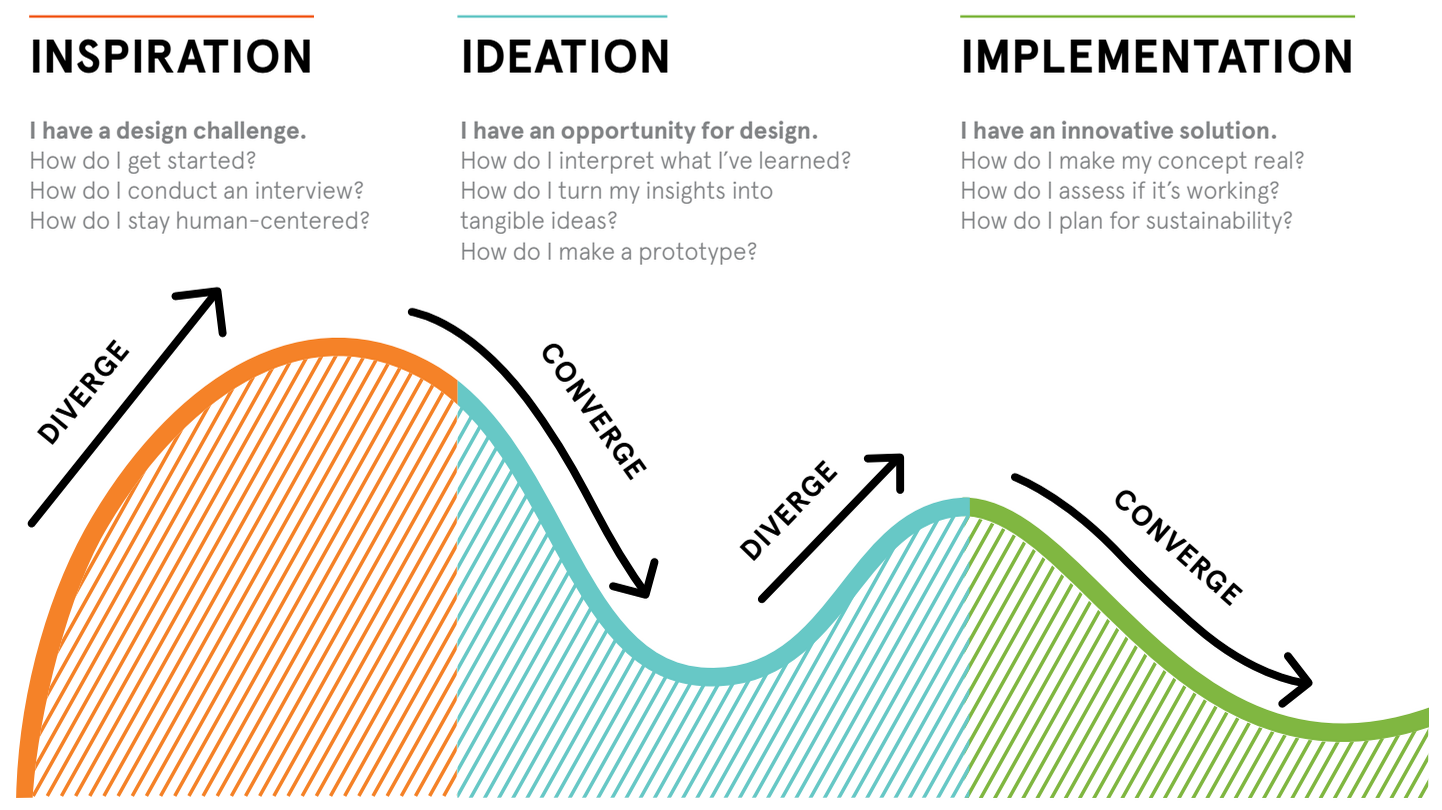
\includegraphics[width=0.6\textwidth]{2}
 	\caption{Trzy zachodzące na siebie fazy procesu Design Thinking'u}
 \end{figure}

\end{itemize}

 
 \subsubsection{Cztero-fazowy proces "Double Dimond"}
 W tym modelu dwa diamenty reprezentują proces zagłębiania problemu, a następnie podejmowanie działań.
  \begin{figure}[h]
 	\centering
 	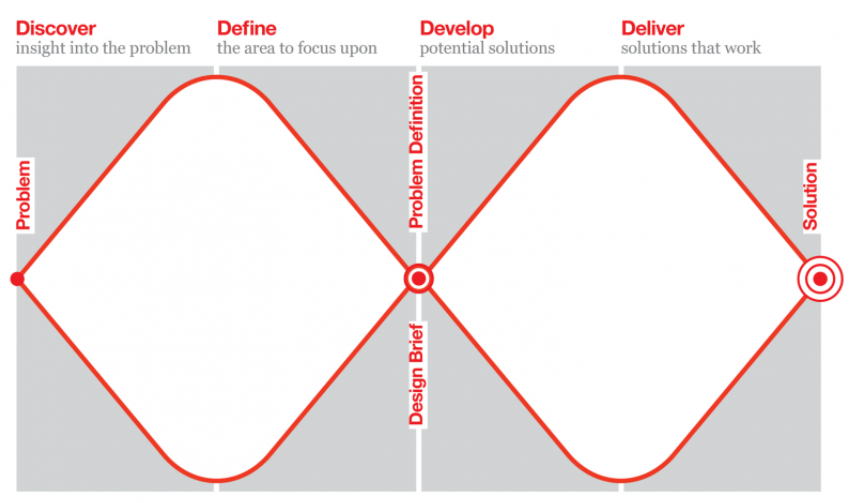
\includegraphics[width=0.6\textwidth]{DoubleDiamond2.PNG}
 	\caption{Cztero-fazowy proces "Double Dimond"}
 \end{figure}
 \begin{itemize}
     \item \textbf{Pierwszy diament}\newline \newline
     Odkrywanie – pomaga zrozumieć problem, a nie tylko założyć jaki on jest. Etap ten wiąże się z rozmawianiem oraz poznawaniem ludzi, których ten problem dotyczy.\newline
     Definiowanie - Informacje zebrane z fazy odkrywania mogą pomóc w zdefiniowaniu wyzwania w inny sposób.\newline
     \item\textbf{Drugi diament}\newline \newline
     Rozwój - zachęca ludzi do udzielania różnych odpowiedzi na jasno zdefiniowany problem, szukania inspiracji z innych źródeł i wspólnego projektowania z szeregiem różnych osób.\newline
     Dostarczanie - obejmuje testowanie różnych rozwiązań na małą skalę, odrzucanie tych, które nie będą działać oraz ulepszanie tych, które mają potencjał.\newline

 
 \end{itemize}

\subsection{Zarządzanie projektem}
\label{sec:zarządzanie_projektem}

\subsubsection{Metody}
\label{sec:narzędzia}
Po analizie wszystkich trzech modeli Design Thinking'u, zdecydowaliśmy się, na podążanie za jedną z metod - Double Diamond. Jest to najbardziej korzystny model w przypadku problememu, z jakim się zetkneliśmy. W tym celu dokładnie zapoznamy się z danym zadaniem, spróbujemy spojrzeć na problem z wielu perspektyw, weźmiemy pod uwagę pomysły i rozwiązania zaproponowane przez każdego członka zespołu. Przanalizujemy oraz wypróbujemy wszystkie możliwości, by finalnie dotrzeć do najbardziej korzystnego rezultatu. 

\vspace{1cm}
\subsubsection{Narzędzia}
\label{sec:narzędzia}


Dostępnych jest wiele narzędzi, które ułatwiają komunikację, usystematyzowanie oraz koordynowanie pracy grupowej. W tym podrozdziale przedstawimy niektóre aplikacje, z którymi można zetknąć się podejmując się wykonywania projektów zespołowych, by następnie dokonać wyboru najbardziej korzystnych w działaniu dla nas narzędzi. \newline \newline

\fbox{Programy do obróbki tekstu:} \newline 

\textbf{LaTeX} \newline
\indent

Zalety:
\begin{itemize}

\item[-]
Wszystkie tytuły sekcji / podpisy tabel, grafik, wykresów są jednakowo formatowane;

\item[-]
Program generuje spis treści;

\item[-]
Pliki PDF generowane przy pomocy LaTeX-a są estetyczne wizualnie;

\item[-]
Możliwość tworzenia wykresów/diagramów za pomocą kodu, bez używania dodatkowych programów; 

\item[-]
LaTeX jest programem o wolnym dostępie – nie musimy za niego płacić;

\item[-]
Pliki LaTeX-a możemy otwierać przy pomocy wielu narzędzi. Możemy używać programów zainstalowanych na komputerze lub wykorzystywać programy internetowe. W przypadku tych drugich istnieje możliwość dzielenia projektu między wiele osób. 
\end{itemize}

\indent

Wady:
\begin{itemize}


\item[-]
Konieczność stosowania odpowiednich bibliotek;

\item[-]
Trudniejsza zmiana np. rodzaju czcionki, marginesów i innych parametrów formatowania pliku w porównaniu do narzędzi typu Word;

\item[-]
Aby korzystać z LaTeX-a trzeba nauczyć się odpowiednich komend oraz poznać składnię.
\end{itemize}

\vspace{1cm}
\textbf{Microsoft Word:}

\indent

Zalety:
\begin{itemize}

\item[-]
Program nie wymaga poznania specjalistycznej składni ani komend;
\item[-]
W łatwy sposób można zmienić parametry np. czcionki, marginesów;
\item[-]
Nie wymaga importowania odpowiednich bibliotek.
\end{itemize}

\indent

Wady:
\begin{itemize}

\item[-]
Wprowadzenie zapisów (symboli) matematycznych jest bardzo trudne;
\item[-]
 Występują problemy z formatowaniem (np. odpowiednie marginesy, akapity);
\item[-]
Podczas przesyłania pliku zdarza się jego deformacja.
\end{itemize}

------------------------------------------------------------\newline \newline
\fbox{Aplikacje komunikacyjne:} \newline 

\textbf{Microsoft Teams} \newline
\indent

Zalety:
\begin{itemize}

\item[-]
Umożliwa komunikację telefoniczną oraz multimedialną, rejestrowanie rozmów ;

\item[-]
Oferuje integracje z duża liczbą innych usług(Word, Excel, Planner, Outlook);

\item[-]
Darmowy dostęp;


\end{itemize}

\indent

Wady:
\begin{itemize}

\item[-]
Mało intuicyjny sposób użytkowania;
\end{itemize}
\vspace{0,8cm}

\textbf{Slack} \newline
\indent

Zalety:
\begin{itemize}

\item[-]
Umożliwa komunikację telefoniczną oraz multimedialną, rejestrowanie rozmów ;

\item[-]
Oferuje integracje z duża liczbą innych usług(Word, Excel, Planner, Outlook);

\item[-]
Darmowy dostęp;


\end{itemize}

\indent

Wady:
\begin{itemize}

\item[-]
Mało intuicyjny sposób użytkowania;
\end{itemize}

\vspace{0,8cm}
\textbf{Skype} \newline
\indent

Zalety:
\begin{itemize}

\item[-]
Umożliwa wykonywanie połączeń telefonicznych oraz video rozmów;

\item[-]
Możliwość udostępniania ekranu rozmówcy;

\end{itemize}

\indent

Wady:
\begin{itemize}

\item[-]
Do korzystania z opcji videokonferencji, która w naszym przypadku jest kluczowa - wymagane wykupienie subskrybcji premium;

\item[-]
Brak połączenia narzędzia z innymi aplikacjami, służącymi do organizacji pracy.
\end{itemize}
------------------------------------------------------------\newline \newline
\fbox{Organizacja pracy:} \newline 

\textbf{Trello} \newline
\indent

Zalety:
\begin{itemize}

\item[-]
Umożliwa wizualne przechowywanie zasobów oraz aktualizowanie na bieżąco dokumentacji ;

\item[-]
Możliwość udostępniania członkom zespołu postępów pracy;

\item[-]
Liczne opcje formatowania tablic;


\end{itemize}
\vspace{1cm}

\textbf{GitHub} \newline
\indent

Zalety:
\begin{itemize}
\item[-]
Kontrola wersji;
	
\item[-]
Struktura branchowa;
	
\item[-]
Miejsce na hosting plików;
	
\item[-]
Możliwość zastosowania w przyszłej karierze zawodowej;
	

Wady:
\item[-]
Wymagane nauczenie się działania systemu
	
\item[-]
Poznanie składni komend
\end{itemize}

------------------------------------------------------------\newline \newline \newline \newline
\vspace{0,5cm}
\textbf{WNIOSKI} \newline

Po analizie wad i zalet powyższych programów oraz aplikacji doszliśmy do następujących wniosków: \newline
Głównym narzędziem służącym do sporządzania sprawozdań będzie \textbf{LaTeX}. Jest to dla naszego zespołu najbardziej korzystny wybór z uwagi na możliwość edycji tekstu przez każdego z członków grupy, w tym samym momencie. W ten sposób możemy dzielić projekt między wszystkimi. Oprócz tego dokument tworzony w LeTeXu wygląda schludnie i estetycznie, nie ulega on formatowaniu na różnych urządzeniach, z których korzystamy. 
Do komunikacji będzie służyła nam aplikacja \textbf{Microsoft Teams}. Główną oraz kluczową w wyborze zaletą, jest możliwość tworzenia telefonicznych konferencji, a także opcja połączenia pracy MSTeams z systemem Git oraz Trello.
Oprócz MSTeams w nagłych i pilnych sytuacjach korzystamy z aplikacji \textbf{Messenger}, która jest w tym momencie najszybszą formą komunikacji. 
Kolejnym narzędziem, które wybraliśmy jest wcześniej wspomniany system kontroli wersji - \textbf{Git}, na platformie github.com.
Będzie służył nam głównie do systematycznej akutalizacji dokumentów oraz możliwości przekazywawnia ich między członkami zespołu. 
Dzięki aplikacji \textbf{Trello} nasza praca pozostanie odpowiednio skoordynowana, a możliwość połączenia aplikacji z Microsoft Teams i otrzymywaniu w ten sposób powiadomień, sprawi, że każdy z członków zespołu wykona dane mu zadanie w odpowiednim czasie. 


\section{Informacje podstawowe}
\label{sec:informacje_podstawowe}

\section{Koncepcja}
\label{sec:koncepcja}

\section{Implementacja}
\label{sec:implementacja}


\section{Uruchomienie}
\label{sec:uruchomienie}


\section{Podsumowanie}
\label{sec:podsumowanie}

\subsection{Tygodniowy harmonogram zadań}



\begin{tabular}{|p{2cm}|p{9cm}|p{3.5cm}|} \hline
Data & Zadanie & Osoba odpowiedzialna \\
\hline
16.03.2020 - 24.03.2020 & Lider zespołu, sporządzenie wniosków  i finalnej częsci raportu & Julia Borysławska \\
\hline
 & Zabranie informacji o Design Thinking'u (wady, zalety, metoda "Trzy fazy") & Sofiia Levchenko\\
\hline
& Zebranie informacji o Design Thinking'u (metody "Double Diamond" i "Pięć kroków") & Joanna Staleńczyk \\
\hline
& Zebranie informacji o narzędziach do obróbki tekstu & Jakub Tarczyński \\
\hline
& Zebranie informacji o narzędziach do organizacji pracy  & Jan Zobiów \\ 

\hline

\end{tabular}





\bibliographystyle{plabbrv} % plplain plabbrv plalpha
\begin{thebibliography}{SYCYfProjekt}
\bibitem{DesignThinking1}
 Visser, W. 2006, The cognitive artifacts of designing, Lawrence Erlbaum Associates.
\bibitem{DesignThinking2}
"Design Thinking: A Beginner’s Guide to the History, Terminologies and Methodologies" by Rhoda Sell \url{https://blog.prototypr.io/design-thinking-a-beginners-guide-to-the-history-terminologies-and-methodologies-e527f7afdcd1}
\bibitem{Proces1}
"The five steps of design thinking" by D.School, Stanford University’s Institute of Design \url{https://dschool-old.stanford.edu/sandbox/groups/designresources/wiki/36873/attachments/74b3d/ModeGuideBOOTCAMP2010L.pdf}
\bibitem{Proces2}
"The three overlapping phases of design thinking" by IDEO. \url{https://www.designkit.org/human-centered-design}
\bibitem{Proces3}
"The four-phased ‘Double Diamond’ process" by the Design Council \url{https://www.designcouncil.org.uk/news-opinion/what-framework-innovation-design-councils-evolved-double-diamond}
\end{thebibliography}

\end{document}
